In this chapter, we first describe the file structure of FDPS Fortran/C interface and overview the way of code development using it. Then, we explain documents and sample codes related to FDPS Fortran/C interface.

%%%%%%%%%%%%%%%%%%%%%%%%%%%%%%%%%%%%%%%%%%%%%%%%%%%%
\section{File structure and overview}
%%%%%%%%%%%%%%%%%%%%%%%%%
\subsection{FDPS}
Source files of FDPS are in the directory \path{src}. FDPS is written in C++ and all the source files related to the standard features are directly under the directory \path{src}. FDPS has extended features and, at present, there are two extended features: ``Particle Mesh" and ``Phantom-GRAPE for x86". The source files related to these features are in the directories \path{src/particle_mesh} and \path{src/phantom_GRAPE_x86}, respectively. These features are used from FDPS as external static libraries. Therefore, users have to build the static libraries when using the extended features. For more details, please see the specification document of FDPS itself (\path{doc/doc_specs_cpp_en.pdf}).
%%%%%%%%%%%%%%%%%%%%%%%%%
\subsection{Fortran interface}
\label{subsec:file_str_ftn_if}
Among the features described in previous section, the standard features (except for some low-level APIs) and the extended feature ``Particle Mesh" are available in Fortran. Users can use these features via Fortran interface programs, which are manually created by the users by executing the script \path{gen_ftn_if.py} in the directory \path{scripts} (see Chap.~\ref{chap:script_spec} for the details of the script). This interface-generating script analyzes \textbf{user-defined types}, which are derived data types that the users must define when using FDPS Fortran interface (see Chap.~\ref{chap:user_defined}), and generate the Fortran interface programs. Thus, \textbf{\Eul{the first thing the users need to do is to implement the user-defined types}}. The reason why the interface programs need to be generated is explained in \S~\ref{subsec:reasons_for_autogen_ftn_if}. Fortran source codes that are required to implement the user-defined types are in the directory \path{src/fortran_interface/modules} and files that are used as blueprint when generating the interface programs are in the directory \path{src/fortran_interface/blueprints}.

Figure~\ref{fig:FDPS_ftn_if_file_str} shows the file structure of the Fortran interface programs and their roles. Four files enclosed by the dashed line (\path{FDPS_module.F90}, \path{FDPS_ftn_if.cpp}, \path{FDPS_Manipulators.cpp}, \path{main.cpp}) are the files to be generated by the script, and the file \path{f_main.F90} corresponds to the user's source codes. In the files enclosed by the dotted line (\path{FDPS_vector.F90}、\path{FDPS_matrix.F90}、\path{FDPS_super_particle.F90}, etc.), several derived data types are defined, which are needed to define the user-defined types and user-defined functions (see Chap.~\ref{chap:overview}). In the following, we explain the role of each interface program.

%%% 図:全体のファイル構成
\begin{figure}[h]
\centering
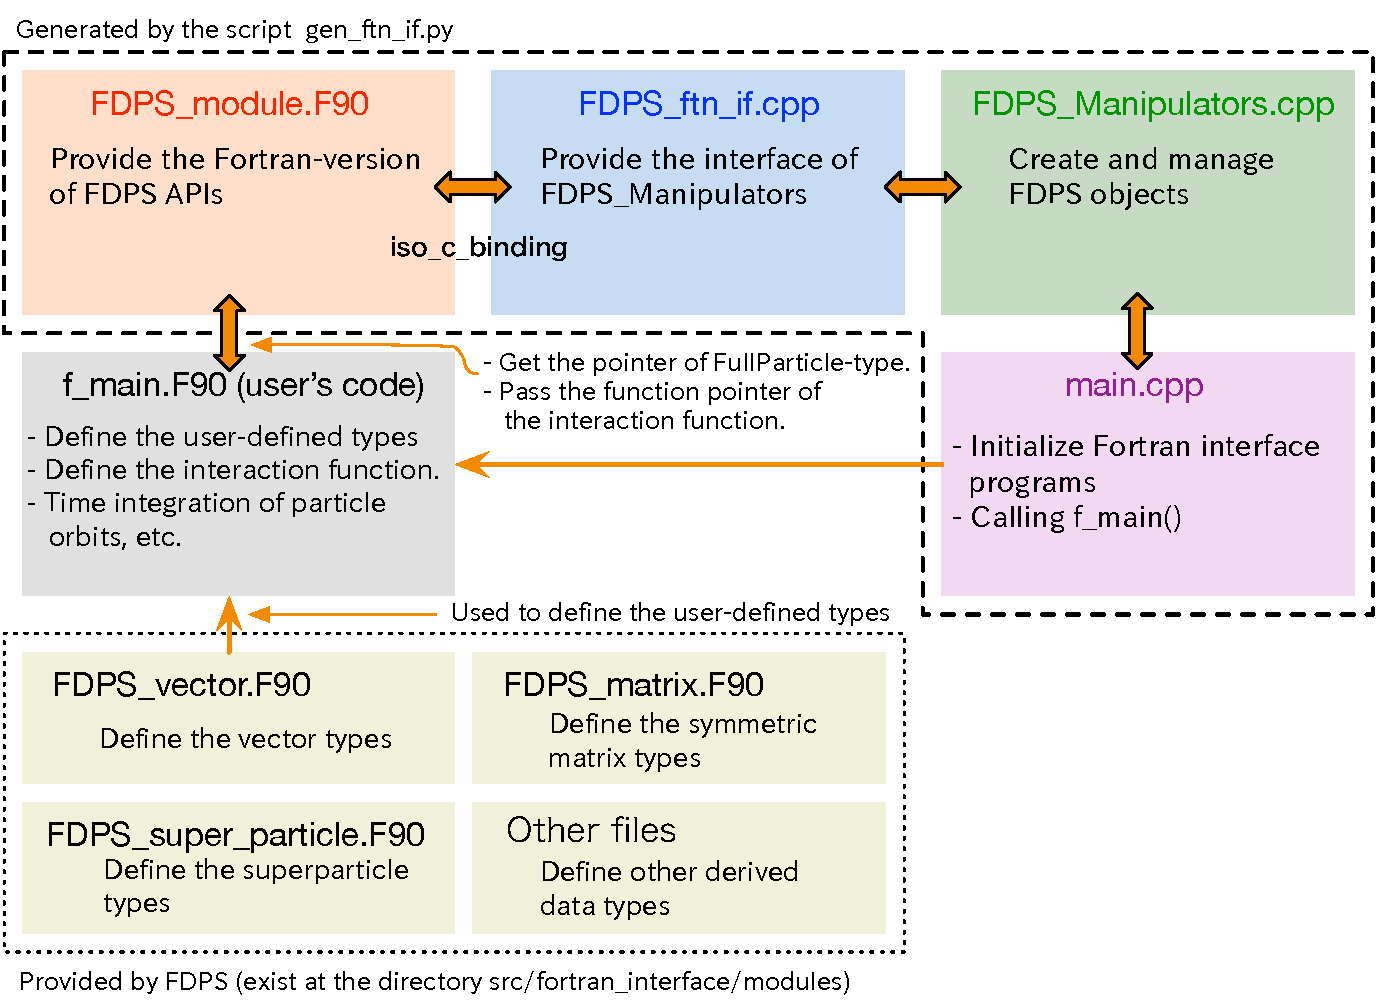
\includegraphics[width=\linewidth]{./fig/FDPS_ftn_if_file_str.pdf}
\caption{File structure of FDPS Fortran interface programs and its relation to user's code}
\label{fig:FDPS_ftn_if_file_str}
\end{figure}

At first, we explain the roles of \path{FDPS_Manipulators.cpp} and \path{main.cpp}. Because FDPS is written in C++, all of C++ objects of DomainInfo class, ParticleSystem class, and TreeForForce class described in Chap.~\ref{chap:overview} must be created and be managed in C++ codes. This task is performed by \path{FDPS_Manipulators.cpp}. By the same reason, we must place the \path{main} function of the user's code in C++ files. Thus, \path{main.cpp} is generated. It calls a Fortran subroutine named \path{f_main()}. Users should prepare a Fortran subroutine \path{f_main()} and must implement all parts of the simulation code inside \path{f_main()}. As described in Chap.~\ref{chap:API_spec_list}, all of C++ objects created in \path{FDPS_Manipulators.cpp} are assigned to Fortran's integer variables. Hence, users also need to manage these objects using integer variables.

Next, we explain the role of \path{FDPS_ftn_if.cpp}. Fortran programs cannot directly call C++ functions. However, a new feature introduced by Fortran 2003 standard (the feature provided by the Fortran module \path{iso_c_binding}) makes it possible that Fortran programs directly call C functions. So, under FDPS Fortran interface, manipulation of FDPS is performed by calling the C interfaces of the functions defined in \path{FDPS_Manipulators.cpp} from a Fortran program. These C interface functions are implemented in \path{FDPS_ftn_if.cpp}.

Finally, we explain the role of \path{FDPS_module.F90}. \path{FDPS_module.F90} provides a derived data type \path{FDPS_controller} for users. This data type is used to call the C interface functions described above. \path{FDPS_controller} is actually a class in Fortran 2003 (a derived data type having member functions or member subroutines) and its member functions provide Fortran interface to FDPS. The list of member functions or Fortran interface is given in Chap.~\ref{chap:API_spec_list}. The class \path{FDPS_controller} is defined in the file \path{FDPS_module.F90} as follows (Listing~\ref{listing:FDPS_module_str}):
\begin{lstlisting}[caption=The structure of \texttt{FDPS\_module.F90},label=listing:FDPS_module_str]
module FDPS_module
   use, intrinsic :: iso_c_binding
   implicit none
   
   !**** FDPS controller
   type, public :: FDPS_controller
   contains
      !
      ! APIs are defined here.
      !
   end type FDPS_controller
   
end module FDPS_module  
\end{lstlisting}
where we have omitted the declaration and implementation parts of the member functions for brevity. Actually, the declaration statements are described in a region between the strings \verb|contains| and \verb|end type FDPS_controller|. For this reason, users should use Fortran interface in the following procedure:
\begin{enumerate}[leftmargin=*,itemsep=-1ex,label=(\arabic*)]
\item Make accessible to the module \path{FDPS_module} by using the \path{use} statement.
\item Create a object of the class \path{FDPS_controller}.
\item Call a member function of the created \path{FDPS_controller} object.
\end{enumerate}
A simplest example of user's code is shown in Listing~\ref{listing:simple_example_ftn_if}:
\begin{lstlisting}[caption=A usage example of Fortran interface,label=listing:simple_example_ftn_if]
subroutine f_main()
   use FDPS_module ! Step (1)
   implicit none
   type(FDPS_controller) :: fdps_ctrl ! Step (2)
   
   ! Call Fortran interface
   call fdps_ctrl%PS_initialize() ! Step (3)
   
end subroutine f_main
\end{lstlisting}
where numbers shown in the comments correspond to the numbers of the procedure described above.

%%%%%%%%%%%%%%%%%%%%%%%%%
\subsection{C interface}
\label{subsec:file_str_c_if}
The features of FDPS that are available in Fortran are also available in C language through C interface programs. The C interface programs are manually created by the users by executing the script \path{gen_c_if.py} in the directory \path{scripts}. This script analyzes C structures that users need to define when using FDPS (we also call them \textbf{user-defined types}) and generates the C interface programs. C header files that are required to implement the user-defined types are in the directory \path{src/c_interface/headers} and files that are used as blueprint when generating the interface programs are in the directory \path{src/c_interface/blueprints}.

Figure~\ref{fig:FDPS_c_if_file_str} shows the file structure of the C interface programs and their roles. Four files enclosed by the dashed line (\path{FDPS_c_if.h}, \path{FDPS_ftn_if.cpp}, \path{FDPS_Manipulators.cpp}, \path{main.cpp}) are the files to be generated by the script, and the file \path{c_main.c} corresponds to the user's source codes. In the files enclosed by the dotted line (\path{FDPS_basic.h}, \path{FDPS_enum.h}, \path{FDPS_vector.h}, \path{FDPS_matrix.h}, \path{FDPS_super_particle.h}, etc.), several structures are defined, which are needed to define the user-defined types and user-defined functions (see Chap.~\ref{chap:overview}). As is clear from the figure, the file structure is very similar to that of the Fortran interface programs. Especially, the files that have the same names as the Fortran interface programs play same roles. In the following, we only describe differences.

%%% Figure:File structure
\begin{figure}[h]
\centering
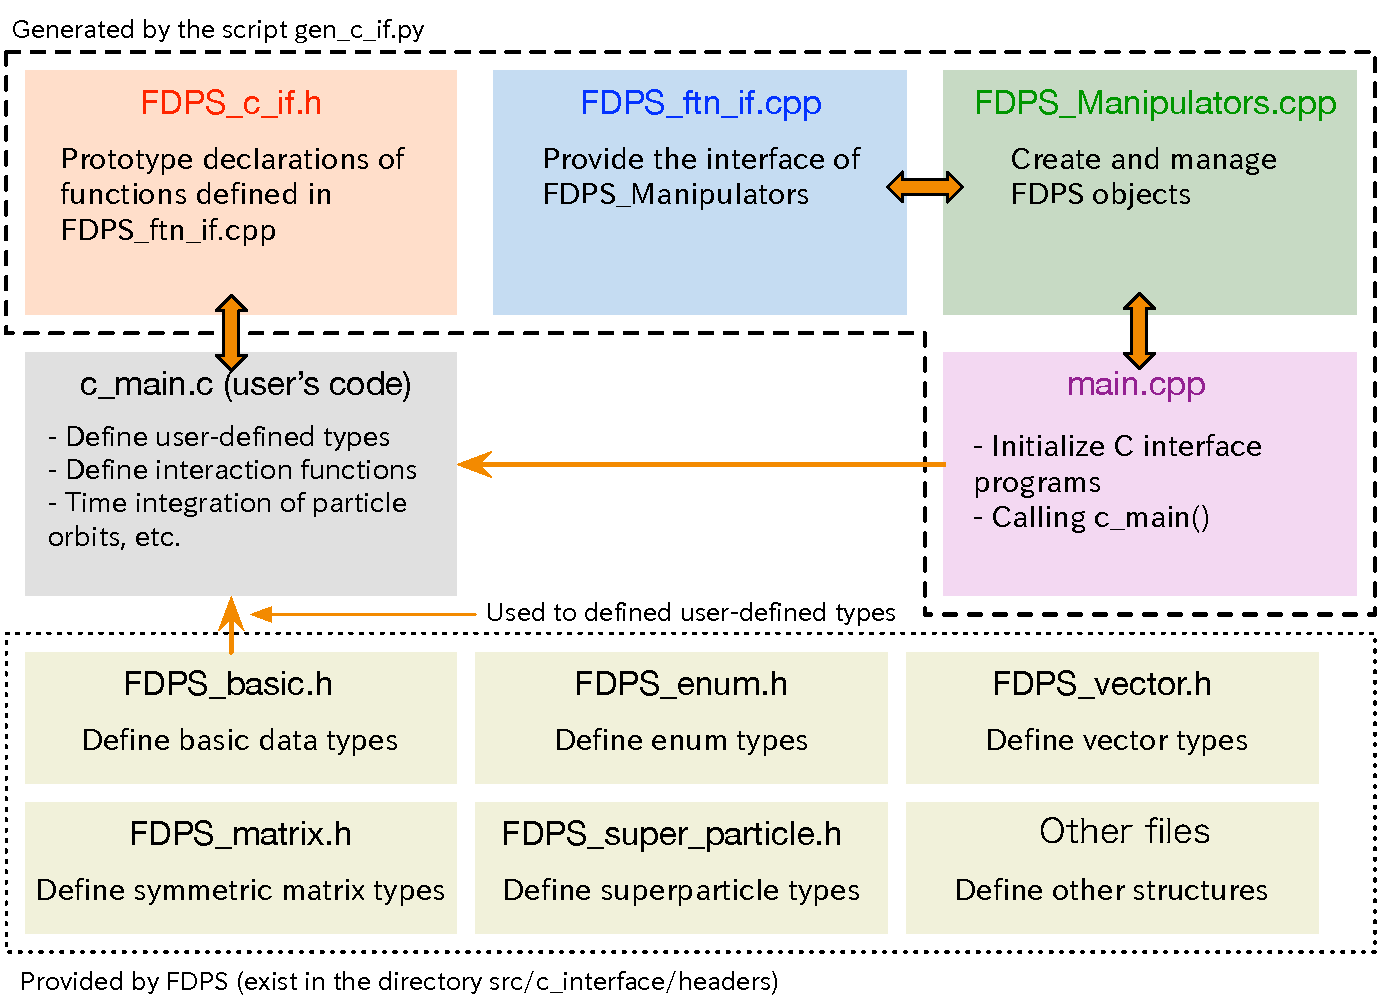
\includegraphics[width=\linewidth]{./fig/FDPS_c_if_file_str.pdf}
\caption{File structure of FDPS C interface programs and its relation to user's code}
\label{fig:FDPS_c_if_file_str}
\end{figure}

\begin{itemize}[leftmargin=*]
\item The \texttt{main} function of the executable is placed in file \path{main.cpp}. In \path{main.cpp}, a \texttt{void} function \path{c_main()} is called. Hence, users must prepare a \texttt{void} function \path{c_main()} and implement all parts of the simulation code inside \path{c_main()}.
\item All of the prototype declarations of APIs for C are described in file \path{FDPS_c_if.h}. Therefore, users must include this file in order to use the features of FDPS. In \path{FDPS_c_if.h}, all the header files described above (e.g. \path{FDPS_basic.h}) are included. Hence, users can use structures provided by FDPS by including this file.
\end{itemize}

%%%%%%%%%%%%%%%%%%%%%%%%%
\subsection{Code development flow with Fortran/C interface}
In this section, we explain a flow of code development with FDPS Fortran/C interface. The following is a rough summary of the flow:
\begin{enumerate}[leftmargin=*,label={[\arabic*]}]
\litem{Define the user-defined types} Implement the user-defined types to generate the interface programs as described in the previous section. The user-defined types must be implemented as  derived data types in Fortran and structures in C. The way to describe the user-defined types is explained in Chap.~\ref{chap:user_defined} in detail.
\litem{Generate  the interface programs} After implementing the user-defined types, generate the interface programs by executing the interface-generating script \path{gen_ftn_if.py} or \path{gen_c_if.py}. If the generation is successfully completed, users can use APIs of FDPS for Fortran/C in user's code. The system requirement of the script and its usage are explained in Chap.~\ref{chap:script_spec}.
\litem{Define the user-defined functions} Implement Fortran subroutine(s) or C \texttt{void} function(s) that describe the details of interaction (the user-defined functions). The way to describe the user-defined functions is explained in Chap.~\ref{chap:user_defined}.
\litem{Write the main part of user's code} Write the main part of a particle simulation code using the user-defined types, the user-defined functions, and APIs of FDPS for Fortran/C. Be aware the following points:
\begin{itemize}
\item Users' code must start and end within a subroutine \path{f_main()} in Fortran or a \texttt{void} function \path{c_main()} in C.
\item The Fortran APIs are provided as the member functions of the Fortran class \path{FDPS_controller}. Hence, users must call the member functions to use the APIs. On the other hand, In C, APIs of FDPS are provided as normal global functions. All the prototype declarations of these functions are described in \path{FDPS_c_if.h}. Hence, users must include this file to use APIs.
\end{itemize}
For concrete examples of code written by using the Fortran interface, please see our sample codes placed in the directory \path{sample/fortran} (see also Chap.~\ref{sec:sample_codes}). Sample codes written by using the C interface are placed in the directory \path{sample/c}.
\litem{Compile} After completing the implementation of user's codes, compile the user's codes to obtain an executable file. As described in the previous sections, the Fortran interface consists of source codes written in C++ and Fortran while the C interface programs consists of source codes written in C++ and C. Therefore, a bit different way of compilation is needed when compared to the case that all the codes are written in a single language. For more information, see Chap.~\ref{chap:compile_and_macro}. Users can configure the setting of some features of FDPS by defining preprocessor macros at the compilation time. We will explain this in Chap.~\ref{chap:compile_and_macro}. When using the extended feature ``Particle Mesh", users must install libraries required by it and must use appropriate compilation options.
\litem{Execute} Run the executable file according to the rule of computer system that a user uses.
\end{enumerate}

%%%%%%%%%%%%%%%%%%%%%%%%%
\subsection{The need for the generation of interface programs}
\label{subsec:reasons_for_autogen_ftn_if}
As described in the previous sections, FDPS Fortran/C interface (sets of APIs of FDPS for Fortran/C) are provided as the form of source codes generated based on user's codes, not as libraries. In this section, we explain the need for generating the interface programs in detail.

As a preparation, we first overview the usage of FDPS in C++ codes. As described in Chap.~\ref{chap:overview} \S~\ref{subsec:things_to_do_by_users}, FDPS allows users to define a particle or an interaction freely. This feature allows FDPS to be applicable for various kinds of particle simulations. In order to realize this feature, FDPS is implemented by using C++ templates.  Roughly speaking, template is a feature of C++ that allows a function to receive data types as actual arguments in addition to usual arguments. Using templates, we can define functions using dummy data types in C++ (a dummy data type does not cause a problem if it is replaced by an actual data type at the compilation time). Also, FDPS is provided as the form of header file. Therefore, when a user uses FDPS in C++, a user first includes the header file of FDPS in the user's code and calls FDPS APIs with passing the particle class(es) defined by the user as the template arguments. During the compilation of the user's code, all the data types used in FDPS APIs are completely determined. Therefore a compiler can compile the code without any problem.

Both Fortran and C do not have a feature corresponding to templates in C++ and therefore we cannot implement functions or subroutines using dummy data types in Fortran or C. This is one reason why we cannot provide FDPS Fortran/C interface as a library. In order to allow users to define particles and interactions freely in Fortran or C, we adopt a system that generates Fortran/C interface programs based on the analysis of derived data types {\small (in Fortran)} or structures {\small (in C)} of particles that are implemented by users.

Another reason comes from the fact that we internally use FDPS written in C++ directly. In order to transfer data between FDPS written in C++ and Fortran/C programs, we need to prepare particle class(es) in the C++ side that are equivalent to the particle types defined by the user in Fortran or C. This also requires the generation of a C++ source code by analyzing derived data types or structures defined by a user.

For the reasons stated above, FDPS Fortran/C interface is provided as the form of the generated source codes.

%%%%%%%%%%%%%%%%%%%%%%%%%%%%%%%%%%%%%%%%%%%%%%%%%%%%
\section{Documents}
All the documents related to FDPS and FDPS Fortran/C interface are in the directory \path{doc}. \path{doc_tutorial_ftn_en.pdf} and \path{doc_tutorial_c_en.pdf} explains basic usage of FDPS Fortran/C interface with using sample codes. \path{doc_specs_ftn_en.pdf} (this document) describes the specification of FDPS Fortran/C interface.

%%%%%%%%%%%%%%%%%%%%%%%%%%%%%%%%%%%%%%%%%%%%%%%%%%%%
\section{Sample codes}
\label{sec:sample_codes}
Sample codes are in the directories \path{sample/fortran} and \path{sample/c}. At present, there are four sample codes: (1) Collision-less gravitational $N$-body simulation code (\path{sample/fortran/nbody} and \path{sample/c/nbody}), (2) SPH (Smoothed Particle Hydrodynamics) code with fixed smoothing length (\path{sample/fortran/sph} and \path{sample/c/sph}), (3) a sample code of $\mathrm{P^{3}M}$ (Particle-Particle Particle-Mesh) method (\path{sample/fortran/p3m} and \path{sample/c/p3m}), and (4) $N$-body/SPH simulation code for galaxy simulation (\path{sample/fortran/nbody+sph} and \path{sample/c/nbody+sph}).
